
\chapter{Konzept}
\label{sec:konzept}
Das Konzept umfasst die Mockups der Formulare, welche in Bonita BPM dargestellt werden sowie den Prozess, welcher modelliert werden soll.

\section{Mockups}
\label{sec:konzept:mockups}
Der Buchungsprozess vom Hotel und Flug Produkt von travel.ch benötigt vier Ansichten, für welche hier Mockups aufgezeigt werden.
Diese wurden mit dem UI Designer von Bonita BPM erstellt (siehe \cref{sec:analyse:bonita:forms:forms} \nameref{sec:analyse:bonita:forms:forms}).

\begin{figure}[H]
	\centering
	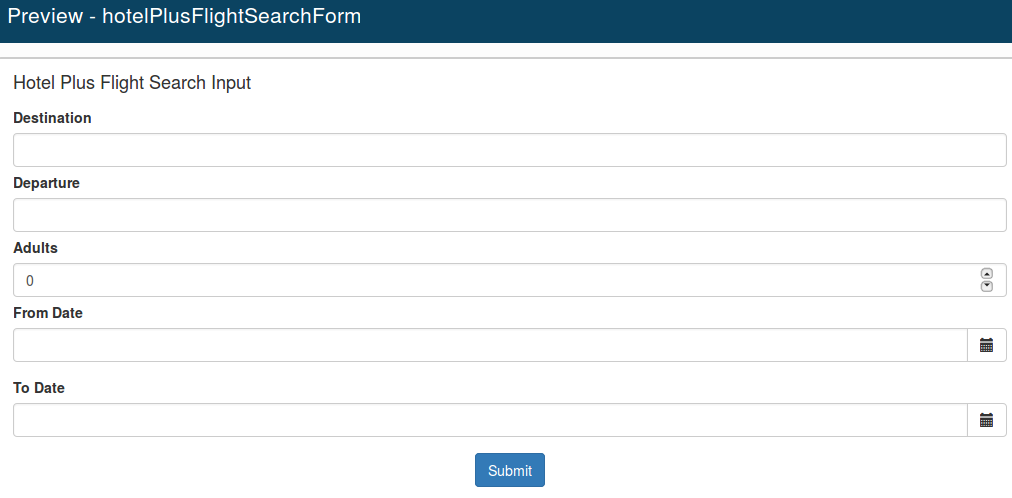
\includegraphics[width=1\textwidth]{images/forms-search.png}
	\caption{Suchformular Mockup}
	\label{fig:konzept:mockups:search}
\end{figure}

Das Suchformular ist vereinfacht dargestellt. Für die Destination muss man einen gültigen Namen eingeben. Auf der Webseite travel.ch wird dem User beim Tippen Vorschläge angezeigt. Dies wurde für dieses Projekt nicht umgesetzt.

Für die Passagiere kann im obigen Formular nur eine Anzahl für die Erwachsenen angegeben werden. Kinder können nicht angewählt werden, da für diese zusätzlich noch das Geburtsdatum angegeben werden muss. Auch die Wahl nach mehreren Zimmern ist nicht möglich. Für die Anzahl der Erwachsenen wird ein Hotelzimmer gesucht.

\begin{figure}[H]
	\centering
	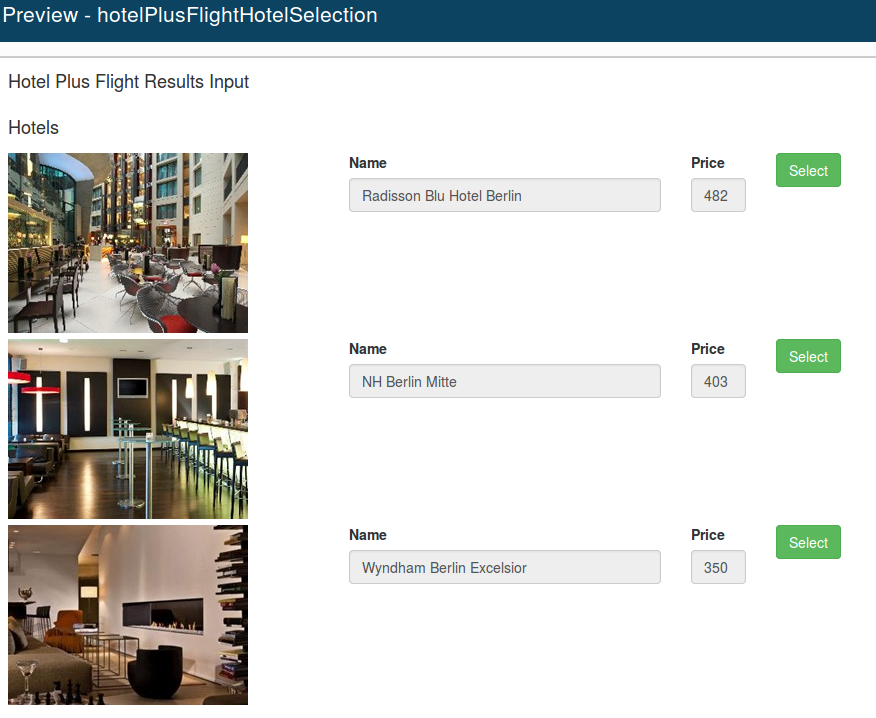
\includegraphics[width=1\textwidth]{images/forms-select-hotel.png}
	\caption{Mockup für die Hotel Suchresultate}
	\label{fig:konzept:mockups:selecthotel}
\end{figure}
Diese Ansicht zeigt ein Foto des Hotels, dessen Namen und den günstigsten Preis. Von der \Gls{glos:api} werden noch mehrere Fotos, eine Geokoordinate für die Anzeige einer Maps, Bewertungsdaten, etc. übermittelt. Diese Informationen werden jedoch nicht angezeigt.

\begin{figure}[H]
	\centering
	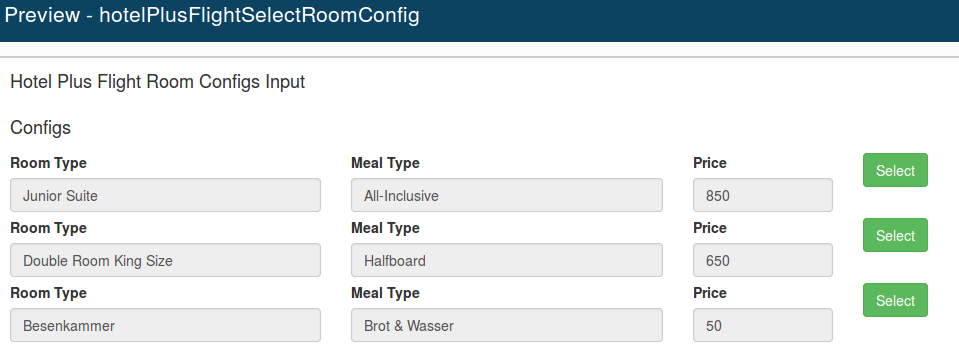
\includegraphics[width=1\textwidth]{images/forms-select-roomconfig.png}
	\caption{Mockup für die Hotelzimmer Konfiguration}
	\label{fig:konzept:mockups:selectroomconfig}
\end{figure}
Auf der travel.ch Seite werden die Zimmer-Konfigurationen als Matrix dargestellt (siehe \cref{fig:recherche:travelch:configuration} \nameref{fig:recherche:travelch:configuration}). In Bonita BPM ist dies jedoch nur sehr umständlich abbildbar. Deshalb wurde die Ansicht vereinfacht und als Liste dargestellt.

\begin{figure}[H]
	\centering
	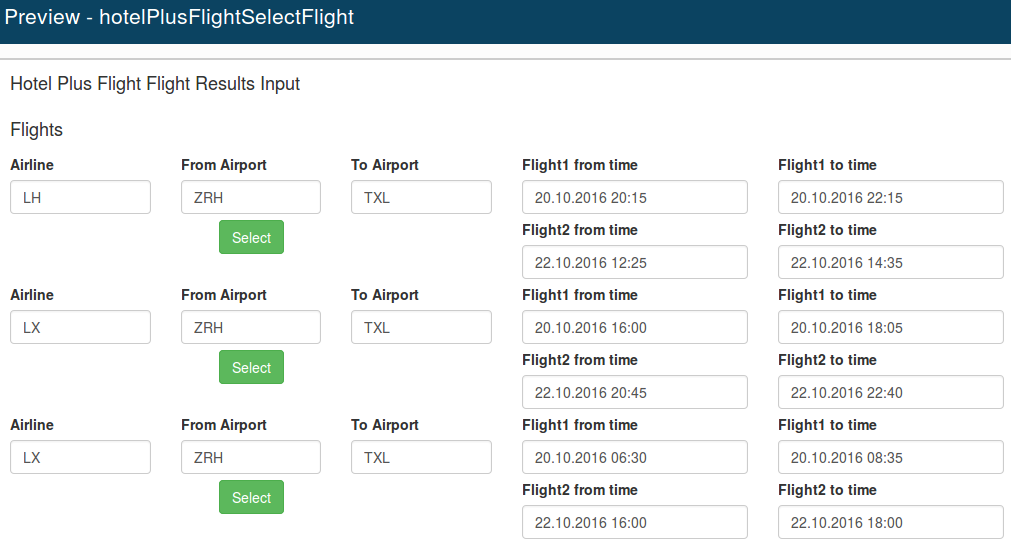
\includegraphics[width=1\textwidth]{images/forms-select-flight.png}
	\caption{Mockup für die Flugresultate}
	\label{fig:konzept:mockups:selectflight}
\end{figure}


\section{Prozess}
\label{sec:konzept:prozess}
Der Process der travel.ch Seite ist linear und wurde im \cref{sec:Recherche:rahmenbedingungen:prozesse} \nameref{sec:Recherche:rahmenbedingungen:prozesse} abgebildet. Für die Modellierung in Bonita BPM wird eine Veränderung vorgenommen.
\begin{figure}[H]
	\centering
	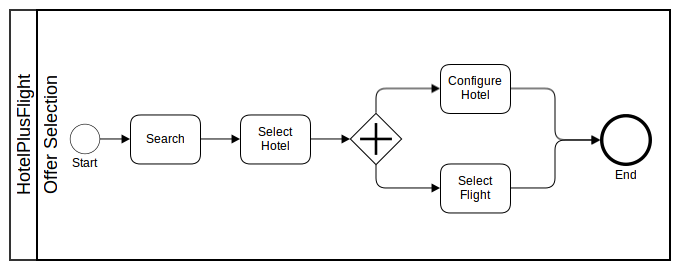
\includegraphics[width=1\textwidth]{images/hotelplusflightbonita.png}
	\caption{Hotel plus Flight BPMN Model für dieses Projekt}
	\label{fig:konzept:mockups:selectflight}
\end{figure}
Die API von travelwindow AG gibt vor, dass zuerst gesucht und ein Hotel ausgewählt wird. Ob danach das Hotel konfiguriert, oder der Flug gewählt wird, ist hinfällig. Dies ist in der API so modelliert, dass im HotelPlusFlightOffer direkt das Formular für die Hotelkonfiguration und die Flugauswahl vorhanden sind (siehe die letzte Anfrage im \cref{sec:analyse:api} \nameref{sec:analyse:api}). Deshalb wurde ein parallel Gateway eingefügt, der diesen Umstand im BPMN abbildet.